% !TeX program = XeLaTeX
% !TeX root = main.tex
% Edit by:xiangyu
\chapter{统计量及其分布\label{cha:5}}
前四章的研究属于概率论的范畴. 我们已经看到, 随机变量及其概率分布全面地描述了随机现象的通解规律性.在概率论的许多问题中, 概率分布通常被假定为已知的, 而一切计算及推理均基于这个已知的分布进行, 在实际问题中, 情况往往并非如此, 看一个例子.
\begin{example}\label{exam5.0.1}
某公司要采购一批产品, 每件产品不是合格品就是不合格品, 但该产品总有一个不合格品率$p$.由此, 若从该批产品中随机抽取一件, 用$X$表示这一件产品的不合格数, 不难看出$X$服从一个二点分布$b(1,p)$,但分布中的参数$p$却是不知道的.显然,  $p$的大小决定了该批产品的质量, 它直接影响采购行为的经济效益.因此, 人们会对$p$提出一些问题, 比如,
\begin{itemize}
\item $p$的大小如何;
\item $p$大概落在什么范围内;
\item 能否认为$p$满足设定要求(如$p\leq0.05$).
\end{itemize}
\end{example}
诸如例~\ref{exam5.0.1} 研究的问题属于数理统计的范畴.接下来我们从统计中最基本的概念——总体和样本开始介绍统计学内容.
\section{总体与样本\label{sec:8.1}}
\subsection{总体与个体\label{ssec:5.1.1}}
在一个统计问题中, 我们把研究对象的全体称为 \textbf{总体}\index{Z!总体}, 构成总体的每个成员称为 \textbf{个体}\index{G!个体}.对多数实际问题, 总体中的个体是一些实在的人或物.比如, 我们要研究某大学的学生身高情况, 则该大学的全体学生构成问题的总体, 而每一个学生即使一个个体.事实上, 每个学生都有许多特征:性别、年龄、身高、体重、名字、籍贯等等, 而在该问题中, 我们关心的只是该校学生的身高如何, 对其他的特征暂不予考虑.这样, 每个学生(个体)所具有的数量指标值——身高就是个体, 而将所有身高全体看成总体.这样一来, 若抛开实际背景, 总体就是一堆数, 这堆数中有大有小, 有的出现的机会多, 有的出现机会小, 因此用一个概率分布去描述和归纳总体是恰当的, 从这个意义看,  \textbf{总体就是一个分布}, 而其数量指标就是服从这个分布的随机变量.以后说``从总体中抽样"与``从分布中抽样"是同一个意思.
\begin{example}
考察某厂的产品质量, 将其产品只分为合格品与不合格品, 并以$0$记合格品, 以$1$记不合格品, 则
\[\text{总体}=\{\text{该厂生产的全部合格品与不合格品}\}=\{\text{由}\;0\;\text{或}\;1\;\text{组成的一堆数}\}.\]
若以$p$表示这堆数中$1$的比例(不合格品率), 则该总体可由一个二点分布表示:
\begin{center}
\begin{tabularx}{0.4\textwidth}{Y|YY}
  X&0&1\\
  \midrule
  P&1-p&p
  \end{tabularx}
\end{center}
不同的$p$反映了总体间的差异. 譬如,两个生产同类产品的工厂的产品总体分布为

\begin{minipage}{0.4\textwidth}
\centering
\begin{tabularx}{\textwidth}{Y|YY}
X&0&1\\
\midrule
P&0.983&0.017
\end{tabularx}
\end{minipage}\hspace{3\ccwd}
\begin{minipage}{0.4\textwidth}
\centering
\begin{tabularx}{\textwidth}{Y|YY}
X&0&1\\
\midrule
P&0.915&0.085
\end{tabularx}
\end{minipage}

我们可以看到,第一个工厂的产品质量优于第二个工厂.实际中,分布中的不合格率是未知的,如何对之进行估计是统计学要研究的问题.
\end{example}
\begin{example}
彩电的彩色浓度是彩电质量好坏的一个重要指标. 20世纪70年代在美国销售的SONY牌彩电有两个产地:美国和日本,两地的工厂是按统一设计方案和相同的生产线生产同一型号SONY彩电,连使用说明书和检验合格的标准也是一样的.其中关于彩色浓度X的标准是:目标值为$m$,公差为$5$,即当$X$在$[m-5,m+5]$内该彩电的热情高于购买美产SONY彩电,原因何在?这就要考察这两个总体有什么差别. 1979年4月17日日本《朝日新闻》刊登调查报告指出,日产SONY彩电的彩色浓度服从正态分布$N(m,(5/3)^2)$,而美产SONY彩电的彩色浓度服从$(m-5,m+5)$上的均匀分布,见图~\ref{fig:5.1.1}.这两个不同的分布代表了不同的总体,其均值相同(都为$m$),但方差不同.若彩色浓度与$m$的距离在$5/3$以内为\Rmnum{1}级品,在$5/3$到$10/3$之间为\Rmnum{2}级品,在$10/3$到$5$之间为\Rmnum{3}级品,其他为\Rmnum{4}级品.于是日产SONY彩电的\Rmnum{1}级品为美产SONY的两倍出头(见表~\ref{table5.1.1}),这就是美国消费者愿意购买日产SONY的主要原因.
\end{example}
\begin{figure}[!htp]
  \centering
\begin{tikzpicture}[scale=1.2]
\begin{scope}[semithick]
\draw(-4,0)--(4,0);
\foreach \x in{-3,...,3}
\draw(\x,0)--(\x,0.1);
\draw[dashed](-3,0)node[below]{$m-5$}--(-3,3.5)(3,0)node[below]{$m+5$}--(3,3.5);
\end{scope}
\draw[samples=100,domain=-4:4,thick]plot(\x,{4*(e^(-(\x)^2/4))+0.1});
\draw(0,0)node[below=1pt]{$m$}--(0,5);
\foreach \x in {-4,...,4}
\coordinate(a\x)at(\x,-0.4);
\begin{scope}[semithick]
\draw[decorate,decoration=brace](a-3)--node[below=1pt]{\Rmnum{4}}(a-4);
\draw[decorate,decoration=brace](a-2)--node[below=1pt]{\Rmnum{3}}(a-3);
\draw[decorate,decoration=brace](a-1)--node[below=1pt]{\Rmnum{2}}(a-2);
\draw[decorate,decoration=brace](a1)--node[below=1pt]{\Rmnum{1}}(a-1);
\draw[decorate,decoration=brace](a2)--node[below=1pt]{\Rmnum{2}}(a1);
\draw[decorate,decoration=brace](a3)--node[below=1pt]{\Rmnum{3}}(a2);
\draw[decorate,decoration=brace](a4)--node[below=1pt]{\Rmnum{4}}(a3);
\draw(-3,1.4)[out=60,in=180]to(-2.5,1.8)--(2.5,1.8)[out=0,in=120]to(3,1.4);
\node[inner sep=0pt,fill=white](a)at(-3,2.5){美产SONY};
\node[inner sep=0pt](b)at(-2.3,3.8){日产SONY};
\draw(a.south)--(-2.5,1.8)(b.east)--(-1,3.2);
\node[inner sep=2pt](c)at(0.5,0.4){$\sigma$};
\draw(1,0)--(c)--(0,0);
\end{scope}
\end{tikzpicture}
  \caption{SONY彩电彩色浓度分布图}\label{fig:5.1.1}
\end{figure}

\begin{table}[!htp]
  \centering
  \caption{各等级彩电的比例(\%)}\label{table5.1.1}
\begin{tabularx}{\textwidth}{Z|Z|Z|Z|Z}
\toprule
等级&\Rmnum{1}&\Rmnum{2}&\Rmnum{3}&\Rmnum{4}\\
\midrule
美产&33.3&33.3&33.3&0\\
\midrule
日产&68.3&27.1&4.3&0.3\\
\bottomrule
\end{tabularx}
\end{table}


在有些问题中,我们对每一研究对象可能要观测两个甚至更多个指标,此时可用多维随机向量及其联合分布来描述总体.这种总体称为多维总体.譬如,我们要了解某校大学生的三个指标: 年龄、身高、月生活支出.则我们可用一个三维随机向量描述该总体.这是一个三维总体,它是多元分析所研究的对象.本书中主要研究一维总体,某些地方也会涉及二维总体.

总体还有有限总体和无限总体,本书将以无限总体作为主要研究对象.
\subsection{样本\label{ssec:5.1.2}}
为了了解总体的分布,我们从总体中随机地抽取$n$个个体,记其指标值为$x_1,x_2,\dotsc,x_n$,则$x_1,x_2,\dotsc,x_n$称为总体的一个 \textbf{样本}\index{Y!样本}, $n$称为 \textbf{样本容量}\index{Y!样本容量},或简称为 \textbf{样本量}\index{Y!样本量},样本中的个体称为 \textbf{样品}\index{Y!样品}.

我们首先指出,样本具有二重性: 一方面,由于样本是从总体中随机抽取的,抽取前无法预知它们的数值,因此,样本是随机变量,用大写字母$X_1,X_2,\dotsc,X_n$表示;另一方面, 样本在抽取以后经观测就有确定的观测值,因此,样本又是一组数值.此时用小写字母$x_1,x_2,\dotsc,x_n$表示是恰当的.简单起见,无论是样本还是其观测值,本书中样本一般均用$x_1,x_2,\dotsc,x_n$表示,读者应能从上下文中加以区别.
\begin{example}\label{exam5.1.3}
啤酒厂生产的瓶装啤酒规定净含量为640 \si{g}.现从某厂生产的啤酒中随机抽取10瓶测定其含量,得到如下结果:
\begin{center}
\begin{tabularx}{0.7\textwidth}{YYYYYYYYYYY}
641&635&640&637&642&638&645&643&639&640
\end{tabularx}
\end{center}
这是一个容量为10的样本的观测值,对应的总体为该厂生产的瓶装啤酒的净含量.
\end{example}
\begin{example} \textbf{(分组样本)}
我们考察某厂生产的某种电子元件的寿命,该厂生产的一级将要生产的所有元件是总体是总体(通常可以认为是无限总体),我们选了100只进行寿命试验,由于一些原因,我们不可能每时每刻对试验进行观察,而只能定期(比如每隔24 \si{h})进行观察,于是,对每个元件,我们只能观察到其寿命落在某个范围内,这就产生了表~\ref{table5.1.2} 所示的一组样本:
\begin{table}
\centering  \caption{100只元件的寿命数据}\label{table5.1.2}
\begin{tabularx}{\textwidth}{YY||YY||YY}
\toprule
\multicolumn{1}{c}{寿命范围}&\multicolumn{1}{c||}{元件数}&
\multicolumn{1}{c}{寿命范围}&\multicolumn{1}{c||}{元件数}&
\multicolumn{1}{c}{寿命范围}&\multicolumn{1}{c}{元件数}\\
\midrule
(0,24]&4&(192,216]&6&(384,408]&4\\
(24,48]&8&(216,240]&3&(408,432]&4\\
(48,72]&6&(240,264]&3&(432,456]&1\\
(72,96]&5&(264,288]&5&(456,480]&2\\
(96,120]&3&(288,312]&5&(480,504]&2\\
(120,144]&4&(312,336]&3&(504,528]&3\\
(144,168]&5&(336,360]&5&(528,552]&1\\
(168,192]&4&(360,384]&1&>552&13\\
\bottomrule
\end{tabularx}
\end{table}

表~\ref{table5.1.2} 中的样本观测值没有具体的数值,只有一个范围,这样的样本称为分组样本\index{F!分组样本}.相应的,例~\ref{exam5.1.3} 中的10个啤酒净含量称为完全样本\index{W!完全样本}.分组样本与完全样本相比在信息上总有损失,这是分组样本的缺点.为了获得更多信息,应尽量设法获得完全样本,在不得已场合可使用分组样本(如上例).但在实际中,在样本量特别大时(如$n\geq100$),又常用分组样本来代替完全样本,这时需要对样本进行分组整理,它能简明扼要地表示样本,使人们能更好地认识总体,这是分组样本的优点.
\end{example}

从总体中抽取样本可以有不同的抽法,为了能由样本对总体作出比较可靠的推断,就希望样本能很好的代表总体.这就需要对抽样方法提出一些要求,最常用的``简单随机样本"有如下两个要求:
\begin{itemize}
\item 样本具有 \textbf{随机性}\index{S!随机性},即要求总体中每一个个体都有同等机会会被选入样本,这便意味着每一样品$x_i$与总体$X$有相同的分布.
\item 样本要有 \textbf{独立性}\index{D!独立性},即要求样本中每一样品的取值不影响其他样品的取值,这意味着$x_1,x_2,\dotsc,x_n$相互独立.
\end{itemize}

用简单抽样方法得到的样本称为 \textbf{简单随机样本}\index{J!简单随机样本},也简称 \textbf{样本}\index{!样本}.除非特别指明,本书中的样本皆为简单随机样本.于是,样本$x_1,x_2,\dotsc,x_n$可以看成是相互独立的具有同一分布的随机变量,其共同分布即为总体分布.

设总体$X$具有分布函数$F(x),x_1,x_2,\dotsc,x_n$为取自该总体的容量为$n$的样本,则样本 \textbf{联合分布函数}\index{L!联合分布函数}为
\[F(x_1,x_2,\dotsc,x_n)=\prod_{i=1}^nF(x_i).\]
对无限总体,随机性与独立性容易实现,困难在于排除有意或无意的认为干扰.对有限总体,只要总体所含个体数很大,特别是与样本量相比很大,则独立性也可基本得到满足.
\begin{example}
设有一批产品共$N$个,需要进行抽样检验以了解其不合格品率$p$,现从中抽出$n$个逐一检查它们是否是不合格的.如果把合格品记为$0$,不合格品记为$1$,则总体为一个二点分布,
\[P(X=1)=p,P(X=0)=1-p,\]
设想样本是一个一个抽出的,结果记为$x_1,x_2,\dotsc,x_n$.如果采取有放回抽样,则$x_1,x_2,\dotsc,x_n$为独立同分布,若采取不放回抽样,这是,第二次抽到不合格品的概率依赖于第一次抽到的是否是不合格品,如果第一次抽到不合格品,则
\[P(x_2=1|x_1=0)=\frac{Np}{N-1}.\]
显然,如此得到的样本不是简单随机样本.但是,当$N$很大时, 我们可以看待上述两种情形的概率都近似等于$p$.所以当$N$很大,而$n$不大(一个经验法则是$n/N\leq0.1$)时可以把该样本近似地看成简单随机样本.
\end{example}

\begin{xiti}
\item 某地电视台想了解某电视栏目(如:每日九点至九点半的体育节目)在该地区的收视率情况,于是委托一家市场咨询公司进行一次电话访查.
\begin{enumerate}
\item 该项研究的总体是什么?
\item 该项研究的样本是什么?
\end{enumerate}
\item 为了了解统计学专业本科毕业生的就业情况,我们调查了某地区30名2000年毕业的统计学专业本科生实习期满后的月薪情况.
\begin{enumerate}
\item 什么是总体?
\item 什么是样本?
\item 样本量是什么?
\end{enumerate}
\item 设某厂大量生产某种产品,其产品不合格率$p$未知,每$m$件产品包装为一盒.为了检查产品的质量,任意抽取$n$盒,查其中的不合格品数,试说明什么是总体,什么是样本,并指出样本的分布.
\item 假设一位运动员在完全相同的条件下重复进行$n$次打靶,试给出总体和样本的统计描述.
\item 某厂生产的电容器的使用寿命服从指数分布,为了解其平均寿命,从中抽出$n$个产品测其实际使用寿命,试说明什么是总体,什么是样本,并指出样本的分布.
\item 美国某高校根据毕业生返校情况记录,宣布该校毕业生的年平均工资为5万美元,你对此有何平均?
\end{xiti}
\section{样本数据的整理与显示\label{sec:5.2}}
\subsection{经验分布函数\label{ssec:5.2.1}}
设$x_1,x_2,\dotsc,x_n$是取自总体分布函数为$F(x)$的样本,若将样本观测值由小到大进行排列,为$x_{(1)},x_{(2)},\dotsc,x_{(n)}$,则$x_ {(1)},x_{(2)},\dotsc,x_{(n)}$称为有序样本\index{Y!有序样本},用有序样本定义如下函数
\begin{equation}\label{eq:5.2.1}
F_n(x)=\begin{cases}
0,&\text{当}x<x_{(1)},\\
k/n,&\text{当}x_{(k)}\leq x<x_{(k+1)},k=1,2\dotsc,n-1,\\
1,&\text{当}x>x_{(n)},
\end{cases}
\end{equation}
则$F_n(x)$是一非减右连续函数,且满足
\[F_n(-\infty)=0\text{和}F_n(+\infty)=1.\]
由此可见, $F_n(x)$是一个分布函数,并称$F_n(x)$为 \textbf{经验分布函数}\index{J!经验分布函数}.
\begin{example}
某食品厂生产听装饮料,现从生产线上随机抽取5听饮料,称得其净重为(单位:\si{g})
\[351\quad347\quad355\quad344\quad351\]
这是一个容量为5的样本,经排序可得有序样本:
\[x_{(1)}=344,\,x_{(2)}=347,\,x_{(3)}=351,\,x_{(4)}=351,\,x_{(5)}=351,\]
其经验分布函数为
\[F_n(x)=\begin{cases}
0,&x<344,\\
0.2,&344\leq x<347,\\
0.4,&347\leq x<351,\\
0.8,&351\leq x<355,\\
1,&x\geq355.
\end{cases}\]
\begin{figure}[!htp]
  \centering
\begin{tikzpicture}[fill=white,draw=black,scale=0.8]
\begin{scope}[semithick,>=Stealth]
\draw[decorate,decoration={snake,segment length=1mm,amplitude=0.5mm}]
(0,0)node[below left]{$O$}--(0.5,0);
\draw[->](-0.5,0)--(0,0)--(0,6)node[left]{$F_n(x)$};
\draw[->](0.5,0)--(8,0)node[below]{$x$};
\end{scope}
\foreach \x in{1,...,5}\draw(0,\x)--(0.1,\x);
\node[left]at(0,1){$0.2$};\node[left]at(0,2){$0.4$};\node[left]at(0,3){$0.6$};
\node[left]at(0,4){$0.8$};\node[left]at(0,5){$1.0$};
\node[below](a)at(1,0){$344$};\node[below](b)at(2.5,0){$347$};
\node[below](c)at(4.5,0){$351$};\node[below](d)at(6.5,0){$355$};
\draw(b)--(2.5,0.1)(c)--(4.5,0.1)(d)--(6.5,0.1);
\draw[ thick](0.5,0)--(1,0)(1,1)--(2.5,1)(2.5,2)--(4.5,2)(4.5,4)--(6.5,4)(6.5,5)--(8,5);
\filldraw(1,0)circle(2pt)(2.5,1)circle(2pt)(4.5,2)circle(2pt)(6.5,4)circle(2pt);
\end{tikzpicture}
  \caption{经验分布函数}\label{fig:5.2.1}
\end{figure}
\end{example}

对每一固定的$x,F_n(x)$是样本中事件``$x_i\leq x$"发生的频率.当$n$固定时, $F_n(x)$是样本的函数,它是一个随机变量,由伯努利大数定律:只要$n$相当大, $F_n(x)$依概率收敛于$F(x)$.更深刻的结果也是存在的,这就是格里纹科定理,下面我们不加证明地加以介绍.
\begin{theorem}{格里纹科定理}{5.2.1}
设$x_1,x_2,\dotsc,x_n$是取自总体分布函数为$F(x)$的样本, $F_n(x)$是其经验分布函数,当$n\to\infty$时,有
\[P\left\{\sup_{-\infty<x<+\infty}|F_n(x)-F(x)|\to0\right\}=1.\]
\end{theorem}

定理~\ref{thm:5.2.1} 表明,当$n$相当大时,经验分布函数是总体分布函数$F(x)$的一个良好的近似.经典的统计学中一切统计推断都以样本为依据,其理由就在于此.
\subsection{频数频率分布表\label{ssec:5.2.2}}
样本数据的整理是统计研究的基础,整理数据的最常用方法之一是给出其频数分布表或频率分布表.我们从一个例子开始介绍.
\begin{example}\label{exam:5.2.2}
为研究某厂工人生产某种产品的能力,我们随机调查了20位工人某天生产的该种产品的数量,数据如下
\begin{align*}
160&&196&&164&&148&&170&\\
175&&178&&166&&181&&162&\\
161&&168&&166&&162&&172&\\
156&&170&&157&&162&&154&
\end{align*}
对这20个数据(样本)进行整理,具体步骤如下
\begin{itemize}
\item  \textbf{对样本进行分组}.首先确定组数$k$,作为一般性的原则,组数通常在$5\sim20$个,对容量较小的样本,通常将其分为5组或6组,容量为100左右的样本可分7到10组,容量为200左右的样本可分9到13组,容量为300左右及以上的样本可分12到20组,目的是使用足够的组来表示数据的变异.本例中只有20个数据,我们将之分为5组,即$k=5$.
\item  \textbf{确定每组组距}.每组区间长度可以相同也可以不同,实用中常选用长度相同的区间以便于进行比较,此时各组区间的长度称为 \textbf{组距}\index{Z!组距},其近似公式为
\[\text{组距}d=\text{样本最大观测值-样本最小观测值)}/\text{组数}\]
本例中,数据最大观测值为196,最小观测值为148,故组距近似为
\[d=\frac{196-148}5=9.6,\]
方便起见,取组距为10.
\item  \textbf{确定每组组限}.各组区间端点为$a_0,a_0+d=a1,a_0+2d=a_2,a_0+2d=a_2,\cdots,a_0+kd=a_k$,形成如下的分组区间
\[(a_0,a_1],(a_1,a_2],\dotsc,(a_{k-1},a_k],\]
其中$a_0$略小于最小观测值, $a_k$略大于最大观测值,本例中可取$a_0=147,a_5=197$,于是本例的分组区间为:
\[(147,157],(157,167],(167,177],(177,187],(187,197],\]
通常可用每组的组中值来代表该组的变量取值,组中值=(组上限$+$组下限)/2.
\item  \textbf{统计样本数据落入每个区间的个数——频数},并列出其频数频率分布表.本例的频数频率分布表见表~\ref{table5.2.1}.从表中可以读出很多信息,如: 40\%的工人产量在157到167之间;产量少于167个的有12人,占60\%;产量高于177的有3人,占15\%.
\end{itemize}
\end{example}
\begin{table}[!htp]
  \centering
  \caption{例~\ref{exam:5.2.2} 的频数频率分布表}\label{table5.2.1}
\begin{tabularx}{0.7\textwidth}{cccccc}
\toprule
组序&分组区间&组中值&频数&频率&累计频率/\%\\
\midrule
1&(147,157]&152&4&0.20&20\\
2&(157,167]&162&8&0.40&60\\
3&(167,177]&172&5&0.25&85\\
4&(177,187]&182&2&0.10&95\\
5&(187,197]&192&1&0.05&100\\
合计&&&20&1&\\
\bottomrule
\end{tabularx}
\end{table}
\subsection{样本数据的图形显示\label{ssec:5.2.3}}
前面我们介绍了频数频率分布的表格形式,它也可以用图形表示,这在许多场合更直观.
\subsubsection{直方图}
频数分布最常用的图形表示是直方图\index{Z!直方图},它在组距相等场合常用宽度相等的长条矩形表示,矩形的高低表示频数的大小.在图形上,横坐标表示所关心变量的取值区间,纵坐标表示频数,这样就得到频数直方图,图~\ref{fig:5.2.2} 画出了例~\ref{exam:5.2.2} 的频数直方图.若把纵轴改成频率就得到频率直方图
为使诸长条矩形面积和为1,可将纵轴取为频率/组距,如此得到的直方图称为单位频率直方图,或简称频率直方图\index{P~频率直方图}.凡此三种直方图的差别仅在于纵轴刻度的选择,直方图本身并无变化.
\begin{figure}[!htb]
\begin{minipage}[b]{0.5\linewidth}
\centering
\begin{tikzpicture}[>=Stealth,yscale=0.5]
\draw[decorate,decoration={snake,segment length=1mm,amplitude=0.5mm}]
(0,0)node[below left]{$O$}--(0.4,0);
\draw(0,0)--(-0.5,0);\draw[->](0,-0.5)--(0,9)node[right]{频数};
\draw[->](0.4,0)--(5,0)node[below]{$x$};
\node[below]at(0.7,0){147};\node[below]at(1.4,0){157};\node[below]at(2.1,0){167};
\node[below]at(2.8,0){177};\node[below]at(3.5,0){187};\node[below]at(4.2,0){197};
\foreach\x in{1,...,8}\draw(0,\x)node[left]{$\x$}--(0.07,\x);
\draw[semithick](0.7,0)--(0.7,4)--(1.4,4)(1.4,0)--(1.4,8)--(2.1,8)--(2.1,0)
(2.1,5)--(2.8,5)--(2.8,0)--(3.5,0)--(3.5,2)--(2.8,2)(3.5,1)--(4.2,1)--(4.2,0)
(0.7,0)--(4.2,0);
\end{tikzpicture}
  \caption{例~\ref{exam:5.2.2} 的频数直方图}\label{fig:5.2.2}
\end{minipage}%
\begin{minipage}[b]{0.5\linewidth}
\centering
\begin{tabular}{r|l}
6&47\\
7&024669\\
8&01223568\\
9&112333566779\\
10&002466788\\
11&2246899\\
12&23568\\
13&3
\end{tabular}\vspace{0.2cm}
\caption{测试成绩的茎叶图}\label{fig:5.2.3}
\end{minipage}
\end{figure}




\subsubsection{茎叶图}
除直方图外,另一种常用的方法是茎叶图\index{J!茎叶图},下面我们从一个例子谈起.
\begin{example}\label{exam:5.2.3}
某公司对应聘人员进行能力测试,测试成绩总分为150分.下面是50位应聘人员的测试成绩(已经过排序):
\begin{align*}
64&&67&&70&&72&&74&&76&&76&&79&&80&&81&\\
82&&82&&83&&85&&86&&88&&91&&91&&92&&93&\\
93&&93&&95&&95&&95&&97&&97&&99&&100&&100&\\
102&&104&&106&&106&&107&&108&&108&&112&&112&&114&\\
116&&118&&119&&119&&122&&123&&125&&126&&128&&133&
\end{align*}
我们用这批数据给出一个茎叶图.把每一个数值分为两部分,前面一部分(百位和十位)称为 \textbf{茎},后面部分(个位)称为  \textbf{叶},如
\begin{center}
\begin{tabularx}{0.7\textwidth}{ZZZZZZZ}
数值&     &分开&     &茎&和&叶\\
112&$\to$&11 | 2&$\to$&11&和&2
\end{tabularx}
\end{center}
然后画一条竖线, \textbf{在竖线的左侧写上茎,右侧写上叶,就形成了茎叶图}.应聘人员测试成绩的茎叶图见图~\ref{fig:5.2.3}.

茎叶图的外观很像横放的直方图,但茎叶图中叶增加了具体的数值,使我们对数据的具体取值一目了然,从面保留了数据中全部的信息.

在要比较两组样本时,可画出它们的 \textbf{背靠背的茎叶图}\index{B!背靠背的茎叶图},这是一个简单直观而有效的对比方法.
\end{example}
\begin{example}\label{exam:5.2.4}
下面的数据是某厂两个车间某天各40名员工生产的产品数量(表~\ref{table5.2.2}).为对其进行比较,我们将这些数据放到一个背靠背茎叶图上(图~\ref{fig:5.2.4}).
\end{example}
\begin{table}[!htp]
  \centering
  \caption{某厂两个车间40名员工的产量}\label{table5.2.2}
\begin{tabularx}{\textwidth}{YYYYYY|YYYYYY}
\toprule
\multicolumn{6}{c|}{甲车间}&\multicolumn{6}{c}{乙车间}\\
\midrule
50&52&56&61&61&62&56&66&67&67&68&68\\
64&65&65&65&67&67&72&72&74&75&75&75\\
67&68&71&72&74&74&75&76&76&76&76&78\\
76&76&77&77&78&82&78&79&80&81&81&83\\
83&85&87&88&90&91&83&83&84&84&84&86\\
86&92&86&93&93&97&86&87&87&88&92&92\\
100&100&103&105&&&93&95&98&107&&\\
\bottomrule
\end{tabularx}
\end{table}
\begin{figure}[!htp]
  \centering
\begin{tabularx}{0.6\textwidth}{R|c|L}
甲车间\hfill620&5&6\hfill 乙车间\\
87775554211&6&67788\\
877664421&7&2245555666889\\
8766532&8&01133344466778\\
73210&9&22358\\
5300&10&7
\end{tabularx}
  \caption{两车间产量的背靠背茎叶图}\label{fig:5.2.4}
\end{figure}
在图~\ref{fig:5.2.4} 中,茎在中间,左边表示甲车间的数据,右边表示乙车间的数据.从茎叶图可以看出,甲车间员工的产量偏于上方,而乙车间员工的产量大多位于中间,乙车间的平均产量要高于甲车间,乙车间各员工的产量比较集中,而甲车间员工的产量则比较分散.
\begin{xiti}
\item 以下是某工厂通过抽样调查得到的10名工人一周内生产的产品数
\[149\quad156\quad160\quad138\quad149\quad153\quad153\quad169\quad156\quad156\]
试由这批数据构造经验分布函数并作图.
\item 下表是经过整理后得到的分组样本
\begin{table}[!htp]
  \centering
\begin{tabularx}{0.9\textwidth}{Z|ZZZZZ}
组序&1&2&3&4&5\\
\midrule
分组区间&(38,48]&(48,58]&(58,68]&(68,78]&(78,88]\\
频数&3&4&8&3&2
\end{tabularx}
\end{table}
试写出此分组样本的经验分布函数.
\item 假若某地区30名2000年某专业毕业生实习期满后的月薪数据如下:
\begin{align*}
909&&1086&&1120&&999&&1320&&1091&\\
1071&&1081&&1130&&1336&&967&&1572&\\
825&&914&&992&&1232&&950&&775&\\
1203&&1025&&1096&&808&&1224&&1044&\\
871&&1164&&971&&950&&866&&738&
\end{align*}
\begin{enumerate}
\item 构造该批数据的频率分布表(分6组);
\item 画出直方图.
\end{enumerate}
\item 某公司对其250名职工上班所需时间进行了调查,下面是其不完整的额率分布表
\begin{center}
\begin{tabularx}{0.8\textwidth}{YY}
\toprule
\multicolumn{1}{Z}{所需时间/\si{min}}&\multicolumn{1}{Z}{频率}\\
\midrule
0\sim10&0.10\\
10\sim20&0.24\\
20\sim30&\\
30\sim40&0.18\\
40\sim50&0.14\\
\bottomrule
\end{tabularx}
\end{center}
\begin{enumerate}
\item 试将频率分布表补充完整.
\item 该公司上班所需时间在半小时以内有多少人?
\end{enumerate}
\item 40种刊物的月发行量如下: (单位:百册)
\begin{align*}
5954&&5022&&14667&&6582&&6870&&1840&&2662&&4508&\\
1208&&3852&&618&&3008&&1268&&1978&&7963&&2048&\\
3077&&993&&353&&14263&&1714&&11127&&6926&&2047&\\
714&&5923&&6006&&14267&&1697&&13876&&4001&&2280&\\
1223&&12579&&13588&&7315&&4538&&13304&&1615&&8612&
\end{align*}
\begin{enumerate}
\item 建立该批数据的频数分布表,取组距为1700百册.
\item 画出直方图.
\end{enumerate}
\item 对下列数据构造茎叶图:
\begin{align*}
472&&425&&447&&377&&341&&369&&412&&419&\\
400&&382&&366&&425&&399&&398&&423&&384&\\
418&&392&&372&&418&&374&&385&&439&&428&\\
429&&428&&430&&413&&405&&381&&403&&479&\\
381&&443&&441&&433&&419&&379&&386&&387&
\end{align*}
\item 根据调查,某集团公司的中层管理人员的年薪数据如下(单位:千元)
\begin{align*}
40.6&&39.6&&43.8&&36.2&&40.8&\\
38.6&&39.6&&40.0&&34.7&&41.7&\\
44.9&&45.4&&37.0&&35.1&&36.7&\\
37.1&&37.7&&39.2&&36.9&&44.5&
\end{align*}
试画出茎叶图.
\end{xiti}
\section{统计量及其分布\label{sec:5.3}}
\subsection{统计量与抽样分布\label{ssec:5.3.1}}
样本来自总体,样本的观测值中含有总体各方面的信息,但这些信息较为分散,有时显得杂乱无章,为将这些分散在样本中的有关总体的信息集中起来以反映总体的各种特征,需要对样本进行加工,表和图是一类加工形式,它是人们从中获得对总体的初步认识.当人们需要从样本获得对总体各种参数的认识时,最常用的加工方法是构造样本的函数,不同的函数反映总体的不同特征.
\begin{definition}{统计量}{tongjiliang}
设$x_1,x_2,\dotsc,x_n$为取自某总体的样本,若样本函数$T=T(x_1,x_2,\dotsc,x_n)$中不含有任何未知参数,则称$T$为 \textbf{统计量}\index{T~统计量}.统计量的分布称为 \textbf{抽样分布}\index{C!抽样分布}.
\end{definition}
按照这一定义,若$x_1,x_2,\dotsc,x_n$为样本,则$\sum_{i=1}^nx_i,\sum_{i=1}^nx_i^2$以及~\ref{ssec:5.2.1} 节中的$F_n(x)$都是统计量.而当$\mu,\sigma^2$未知时, $x_1-\mu,x_1/\sigma$等均不是统计量.必须指出的是: 尽管统计量不依赖于未知参数,但是它的分布一般是依赖于未知参数的.

下面几小节及~\ref{sec:5.4} 节我们介绍一些常见的统计量及其抽样分布.
\subsection{样本均值及其抽样分布\label{ssec:5.3.2}}
\begin{definition}{样本均值}{ybjz}
设$x_1,x_2,\dotsc,x_n$为取自某总体的样本,其算术平均值为 \textbf{样本均值}\index{Y!样本均值},一般用$\bar x$表示,即
\begin{equation}\label{eq:5.3.1}
\bar x=\frac{x_1+\dotsb+x_n}n=\frac1n\sum_{i=1}^nx_i.
\end{equation}
在分组样本场合,样本均值的近似公式为
\begin{equation}\label{eq:5.3.2}
\bar x=\frac{x_1f_1+\dotsb+x_kf_k}n\quad\left(n=\sum_{i=1}^kf_i\right).
\end{equation}
其中$k$为组数, $x_i$为第$i$组的组中值, $f_i$为第$i$组的频数.
\end{definition}
\begin{example}\label{exam:5.3.1}
某单位收集到20名青年人的某月的娱乐支出费用数据:
\begin{align*}
79&&84&&84&&88&&92&&93&&94&&97&&98&&99&\\
100&&101&&101&&102&&102&&108&&110&&113&&118&&125&
\end{align*}
则该月这20名青年的平均娱乐支出为
\[\bar x=\frac1{20}(79+84+\dotsb+125)=99.4.\]
将这20个数据分组可得到如表~\ref{table5.3.1}的频数频率分布:
\end{example}
\begin{table}[!htp]
  \centering
  \caption{~\ref{exam:5.3.1}的频数频率分布表}\label{table5.3.1}
\begin{tabularx}{\textwidth}{ZZZZZ}
\toprule
组序&分组区间&组中值&频数&频率/\%\\
\midrule
1&(77,87]&82&3&15\\
2&(87,97]&92&5&25\\
3&(97,107]&102&7&35\\
4&(107,117]&112&3&15\\
5&(117,127]&122&2&10\\
合计&&&20&100\\
\bottomrule
\end{tabularx}
\end{table}
对表~\ref{table5.3.1} 的分组样本,使用公式~\eqref{eq:5.3.2} 进行计算可得
\[\bar x=\frac1{20}(82\times3+92\times 5+\dotsb+122\times2)=100.\]
我们看到两种计算结果不同.事实上,由于~\eqref{eq:5.3.2} 式未用到真实的样本观测数据,因而给出的是近似结果.

关于样本均值,有如下几个性质.
\begin{theorem}{}{5.3.1}
若把样本中的数据与样本均值之差称为偏差\index{P!偏差},则样本所有偏差之和为$0$, 即$\sum_{i=1}^n(x_i-\bar x)=0$.
\end{theorem}
\begin{proof}
$\sum(x_i-\bar x)=\sum x_i-n\bar x=\sum x_i-n\cdot\big(\sum x_i\big)/n=0$.
\end{proof}

从均值的计算公式看,它使用了所有的数据,而且每一个数据在计算公式中处于平等的地位.所有数据与样本中心的误差被互相抵消,从而样本的所有偏差之和必为零.
\begin{theorem}{}{5.3.2}
数据观察值与均值的偏差平方和最小,即在形如$\sum(x_i-c)^2$的函数中, $\sum(x_i-\bar x)^2$最小,其中$c$为任意给定常数.
\end{theorem}
\begin{proof}
对任意给定的常数$c$,
\begin{align*}
{}&\sum(x_i-c)^2=\sum(x_i-\bar x+\bar x-c)^2\\
=&\sum(x_i-\bar x)^2+n(\bar x-c)^2+
2\sum(x_i-\bar x)(\bar x-c)\\
=&\sum(x_i-\bar x)^2+n(\bar x-c)^2\geq\sum(x_i-\bar x)^2.
\end{align*}

下面考虑样本均值的分布.
\end{proof}
\begin{example}\label{exam:5.3.2}
设有一个由20个数组成的总体,现从该总体抽取容量为5的样本.图~\ref{fig:5.3.1} 画出第一个样本的抽样过程,左侧是该总体,右侧是从总体中随机地抽出的样本,这里一共抽出4个样本,每个样本有5个观测值,我们计算了各个样本的样本均值.从例中可以看到,每一个样本的样本均值都有差别.
\end{example}
\begin{figure}[!htp]
\centering
\begin{tikzpicture}[yscale=0.7,xscale=0.8,inner sep=0.5pt]
\begin{scope}
\node(a)at(0,7){11};\node at(1,7){8};
\node at(0,6.3){12};\node at(1,6.3){13};
\node(b)at(0,5.6){12};\node at(1,5.6){9};
\node at(0,4.9){11};\node at(1,4.9){10};
\node at(0,4.2){9};\node(d)at(1,4.2){11};
\node at(0,3.5){10};\node at(1,3.5){8};
\node at(0,2.8){10};\node at(1,2.8){12};
\node at(0,2.1){11};\node (e)at(1,2.1){9};
\node at(0,1.4){8};\node at(1,1.4){11};
\node (c)at(0,0.7){10};\node at(1,0.7){13};
\end{scope}
\begin{scope}
\node at(2.5,0.9){样本均值};
\node at(4.1,0.9){9.8};\node at(5.6,0.9){10.2};
\node at(7.1,0.9){10.8};\node at(8.6,0.9){10.4};
\node(b1) at(4.1,1.9){8};\node(c1) at(4.1,2.9){10};
\node(e1) at(4.1,3.9){9};\node(d1) at(4.1,4.9){11};
\node(a1) at(4.1,5.9){11};\node at(4.1,6.9){样本1};
\node at(5.6,1.9){9};\node at(5.6,2.9){11};
\node at(5.6,3.9){10};\node at(5.6,4.9){13};
\node at(5.6,5.9){8};\node at(5.6,6.9){样本2};
\node at(7.1,1.9){9};\node at(7.1,2.9){10};
\node at(7.1,3.9){11};\node at(7.1,4.9){11};
\node at(7.1,5.9){13};\node at(7.1,6.9){样本3};
\node at(8.6,1.9){11};\node at(8.6,2.9){10};
\node at(8.6,3.9){10};\node at(8.6,4.9){9};
\node at(8.6,5.9){12};\node at(8.6,6.9){样本4};
\end{scope}
\draw[thick](-0.2,7.3)--(9.2,7.3)(1.6,1.4)--(9.2,1.4)(1.6,6.4)--(9.2,6.4)
(1.6,0.4)--(9.2,0.4);
\foreach \x in{a,b,c,d,e}\draw[-Stealth](\x)--(\x1);
\end{tikzpicture}
  \caption{4个样本的样本均值}\label{fig:5.3.1}
\end{figure}

设想类似抽取样本5、样本6 \raisebox{0.3em}{\tikz\foreach \x in{0.1,0.2,...,0.6}\fill(\x,3)circle(0.7pt);} 每次都计算样本均值,他们之间的差异是由于抽样的随机性引起的.假如无限制地抽下去,这样我们可以得到大量的$\bar x$的值,图~\ref{fig:5.3.2} 就是用这样得到的500个的值所形成的直方图,它反映了$\bar x$的抽样分布.
\begin{figure}[!htp]
  \centering
\begin{tikzpicture}[yscale=0.34,xscale=0.6,>=Stealth,semithick]
\draw[decorate,decoration={snake,segment length=1mm,amplitude=0.5mm}]
(0,0)node[below left]{$O$}--(1,0);
\draw[->](0,0)--(0,12);
\foreach \x in{5,10}\draw(0,\x)node[left]{$\x$}--(0.14,\x);
\draw[->](1,0)--(11.5,0);
\foreach \x/\y in{1/7.5,3/8.5,5/9.5,7/10.5,9/11.5,11/12.5}\draw(\x,0)node[below]{$\y$}--(\x,0.2);
\begin{scope}[xshift=-6.3cm]
\draw[thick](8.1,0)--(8.1,0.5)--(8.5,0.5)--(8.5,0)(8.5,0.3)--(8.9,0.3)--(8.9,0)
--(8.9,0.7)--(9.3,0.7)(9.3,0)--(9.3,3)--(9.7,3)(9.7,0)--(9.7,5)
--(10.1,5)(10.1,0)--(10.1,6)--(10.5,6)(10.5,0)--(10.5,8.2)--(10.9,8.2)(10.9,0)--(10.9,11)
--(11.3,11)(11.3,0)--(11.3,12)--(11.7,12)--(11.7,0)(11.7,10.5)--(12.1,10.5)
(12.1,0)--(12.1,11.7)--(12.5,11.7)--(12.5,0)(12.5,8)--(12.9,8)--(12.9,0)
(12.9,6.7)--(13.3,6.7)--(13.3,0)(13.3,5.4)--(13.7,5.4)--(13.7,0)(13.7,2.2)--(14.1,2.2)
--(14.1,0)(14.1,1.2)--(14.5,1.2)--(14.5,0)(14.5,0.8)--(14.9,0.8)--(14.9,0)--
(14.9,1.1)--(15.3,1.1)--(15.3,0)--(15.3,1.2)--(15.7,1.2)--(15.7,0)(15.7,0.5)--(16.1,0.5)
--(16.1,0);
\end{scope}
\end{tikzpicture}
  \caption{500个样本均值形成的直方图}\label{fig:5.3.2}
\end{figure}

类似地,样本方差也有一个抽样分布,样本标准差也有一个抽样分布.

例~\ref{exam:5.3.2} 中我们给了样本均值的分布一个直观的描述,下面是关于样本均值的抽样分布的一个重要结论.
\begin{theorem}{}{5.3.3}
设$x_1,x_2,\dotsc,x_n$是来自某个总体的样本, $\bar x$为样本均值.
\begin{enumerate}
\item 若总体分布为$N(\mu,\sigma^2)$,则$\bar x$的 \textbf{精确分布}\index{J!精确分布}为$N(\mu,\sigma^2/n)$;
\item 若总体分布位置或不是正态分布,但$E(x)=\mu,\operatorname{Var}(x)=\sigma^2$,则$n$较大时$\bar x$的 \textbf{渐近分布}\index{J!渐近分布}为$N(\mu,\sigma^2)$,常记为$\bar x\dot{\sim}N(\mu,\sigma^2/n)$.这里渐近分布是指$n$较大时的近似分布.
\end{enumerate}
\end{theorem}
\begin{proof}
\begin{enumerate}
\item 利用卷积公式,可得知$\sum_{i=1}^nx_i\sim N(n\mu,n\sigma^2)$,由此可知$\bar x\sim N(\mu,\sigma^2/n)$
\item 由中心极限定理, $\sqrt n(\bar x-\mu)/\sigma\xrightarrow{L}N(0,1)$,这表明$n$较大时$\bar x$的渐近分布为$N(\mu,\sigma^2/n)$,证毕.
\end{enumerate}
\end{proof}
\begin{example}\label{exam:5.3.3}
图~\ref{fig:5.3.3} 给出三个不同总体样本均值的分布.三个总体分别是:
\ding{172}均匀分布、\ding{173}倒三角分布、\ding{174}指数分布,随着样本量的增加,样本均值的抽样分布逐渐向正态分布逼近,他们均值保持不变,而方差则缩小为原来的$1/n$.当样本量为30时,我们看到三个抽样分布都近似于正态分布.下面对之进行说明.
\begin{figure}[!htp]
  \centering
\begin{tikzpicture}[>=Stealth,xscale=0.7,yscale=0.6,thick,samples=100]
\node[align=center] at(1.5,3){$\bar X$的分布\\($n=30$)};
\node[align=center] at(1.5,8){$\bar X$的分布\\($n=5$)};
\node[align=center] at(1.5,11.9){$\bar X$的分布\\($n=2$)};
\node[align=center] at(1.5,15.9){总体分布};
\draw[dashed](0,6)--(12,6)(0,10)--(12,10)(0,14)--(12,14);
\begin{scope}
\draw(3.2,0)--(3.2,0.1)(4.2,0)--(4.2,0.1)(5.2,0)--(5.2,0.1);
\draw[->](3,0)--(3,5.8);
\draw[->](3,0)--(6,0);\node[below]at(3.2,0){$1$};
\node[below]at(4.2,0){$3$};\node[below]at(5.2,0){$5$};
\draw[domain=3.7:4.7]plot(\x,{5.2*(e^(-15*((\x)-4.2)^2))-0.1});
\draw[->](3,6.8)--(6,6.8);
\draw[->](3,6.8)--(3,9.8);\node[below]at(3.2,6.8){$1$};
\node[below]at(4.2,6.8){$3$};\node[below]at(5.2,6.8){$5$};
\draw(3.2,6.8)--(3.2,6.9)(4.2,6.8)--(4.2,6.9)(5.2,6.8)--(5.2,6.9)
(3.7,6.8)--(3.7,6.9)(4.7,6.8)--(4.7,6.9);
\draw[domain=3.4:5]plot(\x,{2.2*(e^(-5*((\x)-4.2)^2))+6.7});
\draw[->](3,10.8)--(6,10.8);
\draw[->](3,10.8)--(3,13.8);\node[below]at(3.2,10.8){$1$};
\node[below]at(4.2,10.8){$3$};\node[below]at(5.2,10.8){$5$};
\draw(3.2,10.8)--(3.2,10.9)(4.2,10.8)--(4.2,10.9)(5.2,10.8)--(5.2,10.9)
(3.7,10.8)--(3.7,10.9)(4.7,10.8)--(4.7,10.9);
\draw(3.2,10.8)--(4.2,13)--(5.2,10.8);
\draw[->](3,14.8)--(6,14.8);
\draw[->](3,14.8)--(3,17.8);\node[below]at(3.2,14.8){$1$};
\node[below]at(4.2,14.8){$3$};\node[below]at(5.2,14.8){$5$};
\draw(3.2,14.8)--(3.2,14.9)(4.2,14.8)--(4.2,14.9)(5.2,14.8)--(5.2,14.9)
(3.7,14.8)--(3.7,14.9)(4.7,14.8)--(4.7,14.9);
\draw(3.2,14.8)--(3.2,17)--node[above]{\ding{172}}(5.2,17)--(5.2,14.8);
\draw[->](6.1,-0.7)--(6.1,18);
\end{scope}
\begin{scope}[xshift=3.4cm]
\draw(3.2,0)--(3.2,0.1)(4.2,0)--(4.2,0.1)(5.2,0)--(5.2,0.1);
\draw[->](3,0)--(3,5.8);
\draw[->](3,0)--(6,0);\node[below]at(3.2,0){$1$};
\node[below]at(4.2,0){$3$};\node[below]at(5.2,0){$5$};
\draw[domain=3.7:4.7]plot(\x,{5.2*(e^(-60*((\x)-4.2)^4))-0.1});
\draw[->](3,6.8)--(6,6.8);
\draw[->](3,6.8)--(3,9.8);\node[below]at(3.2,6.8){$1$};
\node[below]at(4.2,6.8){$3$};\node[below]at(5.2,6.8){$5$};
\draw(3.2,6.8)--(3.2,6.9)(4.2,6.8)--(4.2,6.9)(5.2,6.8)--(5.2,6.9)
(3.7,6.8)--(3.7,6.9)(4.7,6.8)--(4.7,6.9);
\draw[domain=3.2:5.2]plot(\x,{2.2*(e^(-3*((\x)-4.2)^2))+6.7});
\draw[->](3,10.8)--(6,10.8);
\draw[->](3,10.8)--(3,13.8);\node[below]at(3.2,10.8){$1$};
\node[below]at(4.2,10.8){$3$};\node[below]at(5.2,10.8){$5$};
\draw(3.2,10.8)--(3.2,10.9)(4.2,10.8)--(4.2,10.9)(5.2,10.8)--(5.2,10.9)
(3.7,10.8)--(3.7,10.9)(4.7,10.8)--(4.7,10.9);
\draw[domain=3.7:4.7]plot(\x,{2.2*(e^(-3*((\x)-4.2)^2))+10.7});
\draw[domain=3.2:3.7]plot(\x,{1.4*(e^(-20*((\x)-3.57)^2))+10.7});
\draw[domain=4.7:5.2]plot(\x,{1.4*(e^(-20*((\x)-4.83)^2))+10.7});
\draw[->](3,14.8)--(6,14.8);
\draw[->](3,14.8)--(3,17.8);\node[below]at(3.2,14.8){$1$};
\node[below]at(4.2,14.8){$3$};\node[below]at(5.2,14.8){$5$};
\draw(3.2,14.8)--(3.2,14.9)(4.2,14.8)--(4.2,14.9)(5.2,14.8)--(5.2,14.9)
(3.7,14.8)--(3.7,14.9)(4.7,14.8)--(4.7,14.9);
\draw(3.2,14.8)--(3.2,17)--(4.2,14.8)--(5.2,17)--(5.2,14.8);
\node[above]at(4.2,17){\ding{173}};
\draw[->](6.1,-0.7)--(6.1,18);
\end{scope}

\begin{scope}[xshift=6.8cm]
\draw(3,0)node[below]{0}--(3,0.1)(3.5,0)node[below]{$1$}--(3.5,0.1)(4,0)node[below]{2}
--(4,0.1)(4.5,0)node[below]{3}--(4.5,0.1)(5,0)--(5,0.1);
\draw[->](3,0)--(3,5.8);\draw[->](3,0)--(6,0);
\draw[domain=3.7:4.7,xshift=-0.7cm]plot(\x,{5.2*(e^(-15*((\x)-4.2)^2))-0.1});
\draw[->](3,6.8)--(6,6.8);
\draw[->](3,6.8)--(3,9.8);
\draw[yshift=6.8cm](3,0)node[below]{0}--(3,0.1)(3.5,0)node[below]{$1$}--
(3.5,0.1)(4,0)node[below]{2}
--(4,0.1)(4.5,0)node[below]{3}--(4.5,0.1)(5,0)--(5,0.1);
\begin{scope}
\clip(3,6.8)--(3,9.8)--(6,9.8)--(6,6.8)--cycle;
\draw[domain=3.2:5.2,xshift=-0.9cm]plot(\x,{2.2*(e^(-3*((\x)-4.2)^2))+6.7});
\end{scope}
\draw[->](3,10.8)--(6,10.8);
\draw[->](3,10.8)--(3,13.8);
\draw[yshift=10.8cm](3,0)node[below]{0}--(3,0.1)(3.5,0)node[below]{$1$}--
(3.5,0.1)(4,0)node[below]{2}
--(4,0.1)(4.5,0)node[below]{3}--(4.5,0.1)(5,0)--(5,0.1);
\begin{scope}[yshift=4cm]
\clip(3,6.8)--(3,9.8)--(6,9.8)--(6,6.8)--cycle;
\draw[domain=3.2:5.5,xshift=-1.3cm]plot(\x,{2.2*(e^(-4*((\x)-4.4)^2))+6.8});
\end{scope}
\draw[->](3,14.8)--(6,14.8);
\draw[->](3,14.8)--(3,17.8);
\draw[yshift=14.8cm](3,0)node[below]{0}--(3,0.1)(3.5,0)node[below]{$1$}--
(3.5,0.1)(4,0)node[below]{2}
--(4,0.1)(4.5,0)node[below]{3}--(4.5,0.1)(5,0)--(5,0.1);
\node[above]at(4.2,17){\ding{174}};
\draw[out=-80,in=160](3,17)to(4.5,14.8);
\draw[->](6.1,-0.7)--(6.1,18);
\end{scope}
\end{tikzpicture}
  \caption{不同总体样本均值的分布}\label{fig:5.3.3}
\end{figure}

\ding{172}的总体分布为均匀分布$U(1,5)$,该总体的均值和方差分别为$3$和$4/3$,若从该总体抽取样本容量为30的样本,则其样本均值的渐近分布为
\[\bar x_1\dot{\sim}N\left(3,\frac4{3\times40}\right)=N(3,0.21^2).\]

\ding{173}的总体分布的概率密度函数为
\[p(x)=\begin{cases}
(3-x)/4,&1\leq x<3;\\
(x-3)/4,&3\leq x\leq 5;\\
0,&\text{其他}.
\end{cases}\]

这是一个倒三角分布,可以算得其均值与方差分别为3和2,若从该总体抽取样本容量为30的样本,则其样本均值的渐近分布为
\[\bar x_2\dot{\sim} N\left(3,\frac{2}{30}\right)=N(3,0.26^2).\]

\ding{174}的总体分布为指数分布$Exp(1)$,其均值与方差都等于1,若从该总体抽取样本容量为30的样本,则其样本均值$\bar x_3$的分布近似为
\[\bar x_3\dot{\sim}N\left(1,\frac1{30}\right)=N(1,0.18^2).\]

这三个总体都不是正态分布,但其样本均值的分布都十分近似于正态分布,差别表现在均值与标准差上.图~\ref{fig:5.3.3} 所示曲线既展示它们的共同之处,又显示它们之间的差别.
\end{example}
\subsection{样本方差与样本标准差\label{ssec:5.3.3}}
\begin{definition}{}{5.3.3}
设$x_1,x_2,\dotsc,x_n$为取自某总体的样本,则它关于样本均值$\bar x$的平均偏差平方和
\begin{equation}\label{eq:5.3.3}
{s^\ast}^2=\frac1n\sum_{i=1}^n(x_i-\bar x)^2
\end{equation}
称为 \textbf{样本方差}\index{Y!样本方差}.其算术根$s^\ast=\sqrt{{s^\ast}^2}$称为样本标准差.相对样本方差而言,样本标准差通常更有实际意义,因为它与样本均值具有相同的度量单位.在$n$不大时,常用
\begin{equation}\label{eq:5.3.4}
s^2=\frac1{n-1}\sum_{i=1}^n(x_i-\bar x)^2
\end{equation}

作为样本方差(也称 \textbf{无偏方差}\index{W!无偏方差},其含义在第六章讲述),其算术根$s=\sqrt{s^2}$也称为样本标准差.在实际中,$s^2$比${s^\ast}^2$更常用,在以后讲样本方差通常指的是$s^2$.
\end{definition}

在这个定义中, $n$为 \textbf{样本量}\index{Y!样本量}, $\sum_{i=1}^n(x_i-\bar x)^2$称为偏差平方和\index{P!偏差平方和}, $n-1$称为偏差平方和的自由度\index{Z!自由度}.其含义是: 在$\bar x$确定后, $n$个偏差$x_1-\bar x,x_2-\bar x,\dotsc,x_n-\bar x$中只有$n-1$个数据可以自由变动,而第$n$个则不能自由取值,因为$\sum(x_i-\bar x)=0$.

样本偏差平方和有三个不同的表达式:
\begin{equation}\label{eq:5.3.5}
\sum(x_i-\bar x)^2=\sum x_i^2-\frac{\bigl(\sum x_i\bigr)^2}n=\sum x_i^2-n\bar x^2.
\end{equation}
它们都可用来计算样本方差.

在分组样本场合,样本方差的近似计算公式为
\begin{equation}\label{eq:5.3.6}
s^2=\frac1{n-1}\sum_{i=1}^kf_i(x_i-\bar x)^2=\frac1{n-1}\Bigl[\sum_{i=1}^kf_ix_i^2-n\bar x^2\Bigr],
\end{equation}
其中$x_i,f_i$分别为第$i$个区间的组中值和频数, $\bar x$为~\eqref{eq:5.3.2} 中给出的样本均值.
\begin{example}\label{exam:5.3.4}
考察~\ref{exam:5.3.1} 的样本,我们已经算得$\bar x=99.4$,其样本方差与样本标准差分别为
\begin{align*}
s^2&=\frac1{20-1}[(79-99.4)^2+(84-99.4)^2+\dotsb+(125-99.4)^2]133.9368,\\
s&=\sqrt{133.9368}=11.5731,
\end{align*}
对表~\ref{table5.3.1} 的分组样本,我们可以如表~\ref{tab:5.3.2} 计算(样本均值也由分组样本计算):
\begin{table}[!htb]
  \centering
  \caption{分组样本方差的计算表}\label{tab:5.3.2}
\begin{tabularx}{\textwidth}{YYYYY}
\toprule
\text{组中值}x&\text{频数}f&xf&x-\bar x&(x-\bar x)^2f\\
\midrule
82&3&246&-18&972\\
92&5&460&-8&320\\
102&7&714&2&28\\
112&3&336&12&432\\
122&2&244&22&968\\
\text{和}&20&2000&&2720\\
\bottomrule
\end{tabularx}
\end{table}
于是$\bar x=\frac{2000}{20}=100,s^2=\frac{2720}{20-1}=143.16,s=\sqrt{143.16}=11.96$.
\end{example}

下面的定理给出样本均值的数学期望和方差以及样本方差的数学期望,它不依赖于总体的分布形式.这些结果在后面的讨论中是有用的.
\begin{theorem}{}{5.3.4}
设总体$X$具有二阶矩,即$E(X)=\mu,\operatorname{Var}(X)=\sigma^2<+\infty,x_1,x_2,\dotsc,x_n$为从该总体得到的样本, $\bar x$和$s^2$分别是样本均值和样本方差,则
\begin{gather}
E(\bar x)=\mu,\qquad\operatorname{Var}(\bar x)=\sigma^2/n,\label{eq:5.3.7}\\
E(s^2)=\sigma^2.\label{eq:5.3.8}
\end{gather}
\end{theorem}
此定理表明,样本均值的均值与总体均值相同,而样本均值的方差是总体方差的$1/n$.
\begin{proof}
由于
\begin{gather*}
E(\bar x)=\frac1nE\Bigl(\sum_{i=1}^nx_i\Bigr)=\frac{n\mu}n=\mu,\\
\operatorname{Var}(\bar x)=\frac1{n^2}\operatorname{Var}\Bigl(\sum_{i=1}^nx_i\Bigr)
=\frac{n\sigma^2}{n^2}=\frac{\sigma^2}n,
\end{gather*}
故~\eqref{eq:5.3.7} 成立.下证~\ref{eq:5.3.8} ,注意到
\[\sum_{i=1}^n(x_i-\bar x)^2=\sum_{i=1}^nx_i^2-n\bar x^2,\]
而$Ex_i^2=(Ex_i)^2+\operatorname{Var}(x_i)=\mu^2+\sigma^2,E(\bar x^2)=(E\bar x)^2+\operatorname(Var)(\bar x)=\mu^2+\sigma^2/n$,于是
\[E\Bigl(\sum_{i=1}^n(x_i-\bar x)^2\Bigr)=n(\mu^2+\sigma^2)-n(\mu^2+\sigma^2/n)=(n-1)\sigma^2,\]
两边各除以$n-1$,即得~\eqref{eq:5.3.8}.
\end{proof}
\subsection{样本矩及其函数\label{ssec:5.3.4}}
样本均值和样本方差的更一般的推广是样本矩,这是一类常见的统计量.
\begin{definition}{}{5.3.4}
设$x_1,x_2,\dotsc,x_n$是样本,则统计量
\begin{equation}\label{eq:5.3.9}
a_k=\frac1n\sum_{i=1}^nx_i^k
\end{equation}
称为样本$k$阶原点矩.特别,样本一阶原点矩就是样本均值.统计量
\begin{equation}\label{eq:5.3.10}
b_k=\frac1n\sum_{i=1}^n(x_i-\bar x)^k
\end{equation}
称为样本$k$阶中心矩.特别,样本二阶中心矩就是样本方差.
\end{definition}

当总体关于分布中心对称时,我们用$\bar x$和$s$刻画样本特征很有代表性,而当其不对称时,只用$\bar x,s$就显得很不够.为此,需要一些刻画分布形状的统计量.这里我们介绍样本偏度和样本峰度,它们都是样本中心矩的函数.
\begin{definition}{}{5.3.5}
设$x_1,x_2,\dotsc,x_n$是样本,则称统计量
\begin{equation}\label{eq:5.3.11}
\gamma_1=b_3/b_2^{3/2}
\end{equation}
为样本偏度\index{Y!样本偏度}.
\end{definition}
样本偏度$\gamma_1$反映了总体分布密度曲线的对称性信息.如果数据完全对称,则不难看出$b_3=0$.对不对称的数据则$b_3=0$.这里用$b_3$除以$b_2^{3/2}$是为了消除量纲的影响,$\gamma_1$是个相对数,它很好地刻画了数据分布的偏斜方向和程度.如果$\gamma_1$表示样本对称(见图~\ref{fig:5.3.4(a)}),如果$\gamma_1>0$表示样本的右尾长,即样本中有几个较大的数,这反映总体分布是正偏的或右偏的(见图~\ref{fig:5.3.4(b)}),如果$\gamma_1<0$表示分布的左尾长,即样本中有几个特小的数,这反映总体分布是负偏的或左偏的(见图~\ref{fig:5.3.4(c)}).
\begin{definition}{}{5.3.6}
设$x_1,x_2,\dotsc,x_n$是样本,则统计量
\begin{equation}\label{eq:5.3.12}
\gamma_2=\frac{b_4}{b_2^2}-3
\end{equation}
为样本峰度.
\end{definition}

样本峰度$\gamma_2$反映了总体分布密度曲线在其峰值附近的陡峭程度.当$\gamma_2>0$时,分布密度曲线在其峰值附近比正态分布来得陡,称为尖顶型;当$\gamma_2<0$时,分布密度曲线在其峰值附近比正态分布来得平坦,称为平顶型.
\begin{example}\label{exam:5.3.3}
表~\ref{tab:5.3.3} 是两个班(每班50名同学)的英语课程的考试成绩.

下面我们分别计算两个班级的平均成绩、标准差、样本偏度及样本峰度.表
~\ref{tab:5.3.4} 和表~\ref{tab:5.3.5} 分别给出甲班和乙班的计算过程.

可算得两个班的平均成绩、标准差、偏态系数、峰态系数分别为:
\begin{align*}
\begin{gathered}
\bar x_{\text{甲}}=\frac{3790}{50}=75.8,\\
s_{\text{甲}}=\sqrt{\frac{5368}{49}=10.47},\\
\gamma_{1\text{甲}}=\frac{-8908.8/50}{(5368/50)^{3/2}}=-0.16,\\
\gamma_{2\text{甲}}=\frac{1987874.56/50}{(5368/50)^2}-3=0.45,
\end{gathered}\qquad
\begin{gathered}
\bar x_{\text{乙}}=\frac{3790}{50}=75.8,\\
s_{\text{乙}}=\sqrt{\frac{5168}{49}}=10.27,\\
\gamma_{1\text{乙}}=\frac{3571.2/50}{(5168/50)^{3/2}}=0.068,\\
\gamma_{2乙}=\frac{1208706.56/50}{(5168/50)^2}-3=-0.74.
\end{gathered}
\end{align*}
\end{example}
\begin{table}[!htp]
  \centering
  \caption{两个班级的英语成绩}\label{tab:5.3.3}
\begin{tabularx}{\textwidth}{ZZZZ}
\toprule
成绩&组中值&甲班人数$f_{\text{甲}}$&乙班人数$f_{\text{乙}}$\\
\midrule
$90\sim100$&95&5&4\\
$80\sim89$&85&10&14\\
$70\sim79$&75&22&16\\
$60\sim69$&65&11&14\\
$50\sim59$&55&1&2\\
$40\sim49$&45&1&0\\
\bottomrule
\end{tabularx}
\end{table}
\begin{table}[!htp]
  \centering
  \caption{甲班成绩的计算过程}\label{tab:5.3.4}
\begin{tabularx}{\textwidth}{YYYYYY}
\toprule
x&f_{\text{甲}}&x\cdot f_{\text{甲}}&(x-\bar x_{甲})^2f_{\text{甲}}&(x-\bar x_{甲})^3f_{\text{甲}}&(x-\bar x_{甲})^4f_{\text{甲}}\\
\midrule
95&5&475&1843.20&35389.440&679477.2480\\
85&10&850&846.40&7786.880&71639.2960\\
75&22&1650&14.08&-11.264&9.0112\\
65&11&715&1283.04&-13856.832&149653.7856\\
55&1&55&432.64&-8998.912&187 177.3696\\
45&1&45&948.64&-29218.112&899917.8496\\
\midrule
\text{和}&50&3790&5368&-8908.8&1987874.56\\
\bottomrule
\end{tabularx}
\end{table}
\begin{table}[!htp]
  \centering
  \caption{乙班成绩的计算过程}\label{tab:5.3.5}
\begin{tabularx}{\textwidth}{YYYYYY}
\toprule
x&f_{\text{乙}}&x\cdot f_{\text{乙}}&(x-\bar x_{乙})^2f_{\text{乙}}&(x-\bar x_{乙})^3f_{\text{乙}}&(x-\bar x_{乙})^4f_{\text{乙}}\\
\midrule
95&4&380&1474.56&28311.552&543581.7984\\
85&14&1190&1184.96&10901.632&100295.0144\\
75&16&1200&10.24&-8.192&6.5536\\
65&14&910&1632.96&-17635.968&190468.4544\\
55&2&110&865.28&-17997.824&374354.7392\\
\text{和}&50&3790&5168&3571.2&1208706.56\\
\bottomrule
\end{tabularx}
\end{table}
\subsection{次序统计量及其分布}
除了样本矩以外,另一类常见的统计量是 \textbf{次序统计量}\index{C!次序统计量},它在实际和理论中都有广泛的应用.
\subsubsection{定义}
\begin{definition}{}{5.3.7}
设$x_1,x_2,\dotsc,x_n$是取自总体X的样本, $x_{(i)}$称为该样本的第$i$个次序统计量,它的取值是将样本观测值由小到大排列后得到的第$i$个观测值.其中$x_{(1)}=\min\{x_1,\dotsc,x_n\}$称为该样本的 \textbf{最小次序统计量}\index{Z!最小次序统计量}, $x_{(n)}=\max\{x_1,\dotsc,x_n\}$称为该样本的 \textbf{最大次序统计量}\index{Z!最大次序统计量}.
\end{definition}

在一个(简单随机)样本中, $x_1,x_2,\dotsc,x_n$是独立同分布的,而次序统计量$x_{(1)},x_{(2)},\dotsc,x_{(n)}$则既不独立,分布也不相同,看下例.
\begin{example}\label{exam:5.3.6}
设总体$X$的分布为仅取$0,1,2$的离散均匀分布,分布列为
\begin{center}
\begin{tabularx}{0.5\textwidth}{Y|YYY}
x&0&1&2\\
\midrule
p&1/3&1/3&1/3
\end{tabularx}
\end{center}
现从中抽取容量为3的样本,其一切可能取值有$3^3=27$种,现将它们列在表~\ref{tab:5.3.6} 左侧,其右侧相应的次序统计量观测值.
\end{example}
\begin{table}[!htp]
  \centering
  \caption{例~\ref{exam:5.3.6} 中样本取值及其次序统计量}\label{tab:5.3.6}
\begin{tabularx}{\textwidth}{YYY|YYY||YYY|YYY}
\toprule
x_1&x_2&x_3&x_{(1)}&x_{(2)}&x_{(3)}&x_1&x_2&x_3&x_{(1)}&x_{(2)}&x_{(3)}\\
\midrule
0&0&0&0&0&0&1&2&0&0&1&2\\
0&0&1&0&0&1&2&1&0&0&1&2\\
0&1&0&0&0&1&0&2&2&0&2&2\\
1&0&0&0&0&1&2&0&2&0&2&2\\
0&0&2&0&0&2&2&2&0&0&2&2\\
0&2&0&0&0&2&1&1&2&1&1&2\\
2&0&0&0&0&2&1&2&1&1&1&2\\
0&1&1&0&1&1&2&1&1&1&1&2\\
1&0&1&0&1&1&1&2&2&1&2&2\\
1&1&0&0&1&1&2&1&2&1&2&2\\
0&1&2&0&1&2&2&2&1&1&2&2\\
0&2&1&0&1&2&1&1&1&1&1&1\\
1&0&2&0&1&2&2&2&2&2&2&2\\
2&0&1&0&1&2\\
\bottomrule
\end{tabularx}
\end{table}
由于样本取上述每一组观测值的概率相同,都为$1/27$,由此可给出$x_{(1)},x_{(2)},x_{(3)}$的分布列如下:
\begin{center}
\begin{minipage}{0.3\textwidth}
\begin{tabularx}{0.9\textwidth}{Y|YYY}
\toprule
x_{(1)}&0&1&2\\
\midrule
p&\frac{19}{27}&\frac{7}{27}&\frac1{27}\\
\bottomrule
\end{tabularx}
\end{minipage}
\begin{minipage}{0.3\textwidth}
\begin{tabularx}{0.9\textwidth}{Y|YYY}
\toprule
x_{(2)}&0&1&2\\
\midrule
p&\frac{7}{27}&\frac{13}{27}&\frac7{27}\\
\bottomrule
\end{tabularx}
\end{minipage}
\begin{minipage}{0.3\textwidth}
\begin{tabularx}{0.9\textwidth}{Y|YYY}
\toprule
x_{(3)}&0&1&2\\
\midrule
p&\frac{1}{27}&\frac{7}{27}&\frac{19}{27}\\
\bottomrule
\end{tabularx}
\end{minipage}
\end{center}
我们可以清楚地看到这三个次序统计量的分布是不相同的.

进一步,我们可以给出两个次序统计量的联合分布,如, $x_{(1)}$和$x_{(2)}$的联合分布列为
\begin{center}
\begin{tabularx}{\textwidth}{Y|YYY}
\toprule
\multirow{2}*{$x_{(1)}$}&\multicolumn{3}{c}{$x_{(2)}$}\\
\cmidrule{2-4}
&1&2&3\\
\midrule
0&7/27&9/27&3/27\\
1&0&4/27&3/27\\
2&0&0&1/27\\
\bottomrule
\end{tabularx}
\end{center}
因为$P(x_{(1)}=0)P(x_{(2)}=0)=\frac{19}{27}\times\frac7{27}$,而$P(x_{(1)}=0,x_{(2)}=0)=7/27$,两者不等,由此可看出$x_{(1)}$和$x_{(2)}$是不独立的.

接下来我们讨论次序统计量的抽样分布,它们常用在连续总体上,故我们仅就总体$X$的分布为连续情况进行叙述.
\subsubsection{单个次序统计量的分布}
\begin{theorem}{}{5.3.5}
设总体$X$的密度函数为$p(x)$,分布函数为$F(x),x_1,x_2,\dotsc,x_n$为样本,则第$k$个次序统计量$x_{(k)}$的密度函数为
\begin{equation}\label{eq:5.3.13}
p_k(x)=\frac{n!}{(k-1)!(n-k)!}(F(x))^{k-1}(1-F(x))^{n-k}p(x).
\end{equation}
\end{theorem}
\begin{proof}
对任意的实数$x$,考虑次序统计量$x_{(k)}$取值落在小区间$(x,x+\Delta x]$内这一事件,它等价``样本容量为$n$的样本中有1个观测值落在$(x,x+△x]$之间,而有$k-1$个观测值小于等于$x$,有$n一k$个观测值大于$x+△x$'',其直观示意见图~\ref{fig:5.3.5}.
\begin{figure}[!htp]
  \centering
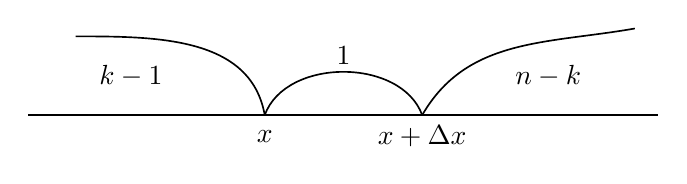
\begin{tikzpicture}[semithick]
\draw(-4,0)--(4,0);\coordinate(a)at(-1,0);\node[below=2pt]at(a){$x$};
\coordinate(b)at(1,0);\node[below]at(b){$x+\Delta x$};
\draw[out=100,in=0](a)to(-3.4,1);
\draw[out=70,in=110](a)to(b);
\node at(0,0.75){$1$};\node at(-2.7,0.5){$k-1$};
\draw[out=60,in=190](b)to(3.7,1.1);
\node at(2.6,0.5){$n-k$};
\end{tikzpicture}
  \caption{$x_{(k)}$取值的示意图}\label{fig:5.3.5}
\end{figure}

样本的每一个分量小于等于$x$的概率为$F(x)$,落入区间$(x,x+\Delta x]$的概率为$F(x+\Delta x)-F(x)$,大于$x+\Delta x$的概率为$1-F(x+\Delta x)$,而将$n$个分量分成这样的三组,总的分法有$\frac{n!}{(k-1)!1!(n-k)!}$种.于是,若以$F_k(x)$记$x_{(k)}$的分布函数,则由多项分布可得
\[F_k(x+\Delta x)-F_k(x)\approx\frac{n!}{(k-1)!1!(n-k)!}(F(x))^{k-1}(F(x+\Delta x)-F(x))(1-F(x+\Delta x))^{n-k},\]
两边除以$\Delta x$,并令$\Delta x\to0$,即有
\begin{align*}
p_k(x)&=\lim_{\Delta x\to0}\frac{F_k(x+\Delta x)-F_k(x)}{\Delta x}\\
&=\frac{n!}{(k-1)!(n-k)!}(F(x))^{k-1}p(x)(1-F(x))^{n-k},
\end{align*}
其中$p_k(x)$的非零区间与总体的非零区间相同.特别,令$k=1$和$k=n$即得到最小次序统计量$x_{(1)}$和最大次序统计量$x_{(n)}$的密度函数分别为:
\begin{gather}
p_1(x)=n\cdot(F(x))^{n-1}p(x),\label{eq:5.3.14}\\
p_n(x)=n\cdot(1-F(x))^{n-1}p(x).\label{eq:5.3.15}
\end{gather}
\end{proof}
\begin{example}\label{exam:5.3.7}
设总体密度函数为
\[p(x)=3x^2,\quad0<x<1,\]
现从该总体抽得一个容量为5的样本,试计算$P(x_{(2)}<1/2)$.
\end{example}
\begin{solution}
我们首先应求出$x_{(2)}$的分布.由总体密度函数不难求出总体分布函数为
\[F(x)=\begin{cases}
0,&x\leq0;\\
x^3,&0<x<1\\
1,&x\geq1.
\end{cases}\]
由公式~\eqref{eq:5.3.8} 可以得到$x_{(2)}$的密度函数为
\begin{align*}
p_2(x)&=\frac{5!}{(2-1)!(5-2)!}(F(x))^{2-1}p(x)(1_F(x))^{5-2}\\
&=20\cdot x^3\cdot3x^2\cdot(1-x^3)^3=60x^5(1-x^3)^3,\quad 0<x<1,
\end{align*}
于是
\begin{align*}
P(x_{(2)}<1/2)&=\int_0^{1/2}60x^5(1-x^3)^3\dd x\\
&=\int_0^{1/8}20y(1-y)^5\dd y=\int_{7/8}^120(z^3-z^4)\dd z\\
&=5(1-(7/8)^4)-4(1-(7/8)^5)=0.1207.
\end{align*}
\end{solution}
\begin{example}\label{exam:5.3.8}
设总体分布为$U(0,1),x_1,x_2,\dotsc,x_n$为样本,则其第$k$个次序统计量的密度函数为
\[p_k(x)=\frac{n!}{(k-1)!(n-k)!}x^{k-1}(1-x)^{n-k},\quad0<x<1,\]
这就是\S\ref{sec:2.5} 中介绍的贝塔分布$Be(k,n-k+1)$,从而有$E(x_{(k)})=\frac k{n+1}$.
\end{example}
\subsubsection{多个次序统计量的联合分布}
下面我们讨论任意二个次序统计量的联合分布.对三个或三个以上次序统计量的分布可参照进行.
\begin{theorem}{}{5.3.6}
在定理~\ref{thm:5.3.5} 的记号下,次序统计量$(x_{(i)},x_{(j)})(i<j)$的联合分布密度函数为
\begin{equation}\label{eq:5.3.16}
p_{ij}(y,z)=\frac{n!}{(i-1)!(j-i-1)!(n-j)!}[F(y)]^{i-1}[F(z)-F(y)]^{j-i-1}
\cdot[1-F(z)]^{n-j}p(y)p(z),\quad y\leq z,
\end{equation}
\end{theorem}
\begin{proof}
对正能量$\Delta y,\Delta z$以及$y<z$,事件``$x_{(i)}\in(y,y+\Delta y],x_{(j)}\in(z,z+\Delta z]$''可以表示为``容量为$n$的样本$x_1,\dotsc,x_n$中有$i-1$个观测值小于等于$y$,一个落入区间$(y,y+\Delta y],j-i-1$个落入区间$(y+\Delta y,z]$,一个落入区间$(z,z+\Delta z]$,而余下$n-j$个大于$z+\Delta z$''(见图~\ref{fig:5.3.6}).
\begin{figure}[!htp]
  \centering
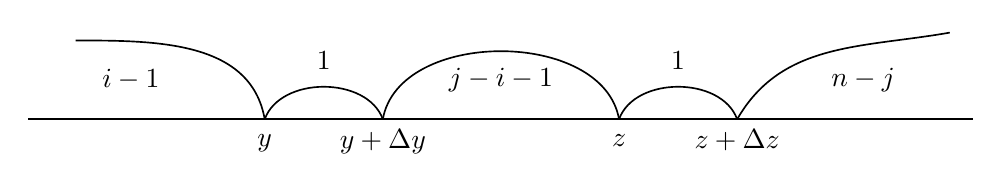
\begin{tikzpicture}[semithick]
\draw(-6,0)--(6,0);
\coordinate(a) at(-3,0);\coordinate(b)at(-1.5,0);
\coordinate(c)at(1.5,0);\coordinate(d)at(3,0);
\node[below=2pt]at(a){$y$};\node[below]at(b){$y+\Delta y$};
\node[below=2pt]at(c){$z$};\node[below]at(d){$z+\Delta z$};
\draw[out=100,in=0](a)to(-5.4,1);
\draw[out=70,in=110](a)to(b);\draw[out=70,in=110](c)to(d);
\node at(-2.25,0.75){$1$};\node at(-4.7,0.5){$i-1$};
\draw[out=60,in=190](d)to(5.7,1.1);
\node at(4.6,0.5){$n-j$};\node at(0,0.5){$j-i-1$};
\draw[out=80,in=100](b)to(c);
\node at(2.25,0.75){$1$};
\end{tikzpicture}
  \caption{$x_{(i)}$与$x_{(j)}$取值的示意图}\label{fig:5.3.6}
\end{figure}

于是由多项分布可得
\begin{align*}
{}&P(x_{(i)}\in(y,y+\Delta y),x_{(j)}\in(z,z+\Delta z))\\
\approx&\frac{n!}{(i-1)!1!(j-i-1)!1!(n-j)!}[F(y)]^{i-1}p(y)\Delta y[F(z)-F(y+\Delta y)]^{j-i-1}p(z)\Delta z[1-F(z+\Delta z)]^{n-j},
\end{align*}
考虑到$F(x)$的连续性,当$\Delta y\to0,\Delta z\to0$时有$F(y+\Delta y)\to F(y),F(z+\Delta z)\to F(z)$,于是
\begin{align*}
p_{ij}(y,z)&=\lim_{\Delta y\to0,\Delta z\to0}
\frac{x_{(i)}\in(y,y+\Delta y),x_{(j)}\in(z,z+\Delta z)}{\Delta y\cdot\Delta z}\\
&=\frac{n!}{(i-1)!(j-i-1)!(n-j)!}[F(y)]^{i-1}[F(z)-F(y)]^{j-i-1}[1-F(z)]^{n-j}p(y)p(z).
\end{align*}
定理得证.
\end{proof}

在实际问题中会用到一些次序统计量的函数,如$R_n=x_{(n)}-x_{(1)}$称为 \textbf{样本极差}\index{Y!样本极差},是一个很常用的统计量,要推导这个统计量的分布原则上并不难,我们只要使用定理~\ref{fig:5.3.6} 以及第三章讲过的随机变量函数的分布求法即可解决.但它们的分布常用积分表示,只在很少几种场合可用初等函数表示,下面是一个样本极差的分布可用初等函数表示的例子.
\begin{example}
设总体分布为$U(0,1),x_1,x_2,\dotsc,x_n$为样本,则$(x_{(1)},x_{(n)})$的联合密度函数为
\[p_{1,n}(y,z)=n(n-1)(z-y)^{n-2},\quad 0<y<z<1,\]
令$R=x_{(n)}-x_{(1)}$,由$R>0$可以推出$0<x_{(1)}=x_{(n)}-R\leq1-R$,则
\[p_R(r)=\int_0^{1-r}n(n-1)[(y+r)-y]^{n-2}\dd y=n(n-1)r^{n-2}(1-r).\]
这正是参数为$(n-1,2)$的贝塔分布.
\end{example}
\subsection{样本分位数与样本中位数}
 \textbf{样本中位数}\index{Y!样本中位数}也是一个很常见的统计量,它也是次序统计量的函数,通常如下定义.设$x_{(1)},\dotsc,x_{(n)}$是有序样本,则 \textbf{样本中位数}\index{Y!样本中位数} $m_{0,5}$定义为
\[m_{0,5}=\begin{cases}
x_{\left(\frac{n+1}2\right)},&n\;\text{为奇数}\\
\frac12\left(x_{(n/2)}+x_{(n/2+1)}\right),&\;\text{为偶数}.
\end{cases}\]
譬如,若$n=5$,则$m_{0,5}=x_{(3)}$,若$n=6$,则$m_{0,5}=\frac12(x_{(3)}+x_{(4)})$.

更一般地,样本$p$分位数$m_p$可如下定义:
\[m_p=\begin{cases}
x_{[np+1]},&\text{若}\;np\;\text{不是整数};\\
\frac12(x_{np}+x_{(np+1)}),&\text{若}\;np\;\text{是整数}.
\end{cases}\]
譬如,若$n=10,p=0.35$,则$m_{0.35}=x_{(4)}$,若$n=20,p=0.45$,则$m_{0.45}=\frac12(x_{(9)}+x_{(10)})$.

对多数总体而言,要给出样本p分位数的精确分布通常不是一件容易的事.幸运的是当$n\to+\infty$时样本$p$分位数的渐近分布有比较简单的表达式,我们这里不加证明地给出如下定理.
\begin{theorem}{}{5.3.7}
设总体密度函数为$p(x),x_p$为其$p$分位数, $p(x)$在$x_p$处连续且$p(x_p)>0$,则当$n\to+\infty$时样本$p$分位数$m_p$的渐近分布为
\begin{equation}\label{eq:5.3.17}
m_p\dot{\sim}N\left(x_p,\frac{p(1-p)}{n\cdot p^2(x_p)}\right).
\end{equation}
特别,对样本中位数,当$n\to+\infty$时近似地有
\begin{equation}\label{eq:5.3.18}
m_{0.5}\dot{\sim}\left(x_{0.5},\frac1{4n\cdot p^2(x_{0.5})}\right).
\end{equation}
\end{theorem}
\begin{example}
设总体为柯西分布,密度函数为
\[p(x;\theta)=\frac1{\pi(1+(x-\theta)^2)},\quad -\infty<x<+\infty,\]
其分布函数为
\[F(x;\theta)=\frac12+\frac1\pi\arctan(x-\theta).\]
不难看出$\theta$是该总体的分位数,即$x_{0.5}=\theta$.设$x_1,\dotsc,x_n$是来自该总体的样本,当样本量$n$较大时,样本中位数$m_{0.5}$的渐近分布为
\[m_{0.5}\dot{\sim}N\left(\theta,\frac{\pi^2}{4n}\right).\]
\end{example}
通常,样本均值在概括数据方面具有一定的优势.但样本均值也有其不足之处.设我们有5个数$3,5,9,10,13$,则其均值为$(3+5+9+10+13)/5=8$.如果我们不小心将13错输入为133(比如在计算机输入时将3连按2下),则均值即变为$(3+5+9+10+133)/5=32$.这说明均值受极端数值影响较大,与之相对应,中位数则不受极端值的影响,因此,当数据中含有极端值时,使用中位数比使用均值更好,中位数的这种抗干扰性在统计中称为具有 \textbf{稳健性}\index{W!稳健性}.
\subsection{五数概括与箱线图}
次序统计量的应用之一是五数概括\index{W!五数概括}与箱线图\index{X!箱线图}.在得到有序样本后,容易计算如下五个值: 最小观测值$x_{\min}=x_{(1)}$;最大观测值$x_{\max}=x_{(n)}$,中位数$m_{0.5}$,第一4分位数$Q_1=m_{0.25}$和第三4分位数$Q_3=m_{0.75}$.所谓五数概括就是指用这五个数:
\[x_{\min},\quad Q_1,\quad m_{0.5},\quad Q_3,x_{\max}\]
来大致描述一批数据的轮廓.
\begin{example}\label{exam:5.3.11}
表~\ref{tab:5.3.7} 是某厂160名销售入员某月的销售量数据的有序样本,由该批数据可计算得到$x_{\min}=45,x_{\max}=319,m_{0.5}=181,Q_1=144,Q_3=212$.
\end{example}
\begin{table}[!htp]
  \centering
  \caption{某厂160名销售员的月销售量的有序样本}\label{tab:5.3.7}
\begin{tabularx}{\textwidth}{YYYYYYYYYY}
\toprule
45&74&76&80&87&91&92&93&95&96\\
98&99&104&106&111&113&117&120&122&122\\
124&126&127&127&129&129&130&131&131&133\\
134&134&135&136&137&137&139&141&141&143\\
145&148&149&149&149&150&150&153&153&153\\
153&154&157&160&160&162&163&163&165&165\\
167&167&168&170&171&172&173&174&175&175\\
176&178&178&178&179&179&179&180&181&181\\
181&182&182&185&185&186&186&187&188&188\\
188&189&189&191&191&191&192&192&194&194\\
194&194&195&196&197&197&198&198&198&199\\
200&201&202&204&204&205&205&206&207&210\\
214&214&215&215&216&217&218&219&219&221\\
221&221&221&221&222&223&223&224&227&227\\
228&229&232&234&234&238&240&242&242&242\\
244&246&253&253&255&258&282&290&314&319\\
\bottomrule
\end{tabularx}
\end{table}
五数概括的图形表示称为箱线图,由箱子和线段组成.图~\ref{fig:5.3.7} 是例~\ref{exam:5.3.11} 中样本数据的箱线图,其作法如下:

(1)画一个箱子,其两侧恰为第一4分位数和第三4分位数,在中位数位置上画一条竖线,它在箱子内.这个箱子包含了样本中50\%的数据;

(2)在箱子左右两侧各引出一条水平线,分别至最小值和最大值为止.每条线段包含了样本中25\%的数据.
\begin{figure}[!htp]
  \centering
\begin{tikzpicture}[scale=3]
\draw(0,0)--(3.5,0);
\draw[dashed](0.3,0.7)--(0.3,0)node[below]{45};
\draw[dashed](3.2,0.7)--(3.2,0)node[below]{319};
\draw[semithick](0.3,0.7)--(1.2,0.7)(2.3,0.7)--(3.2,0.7);
\draw[semithick](1.2,0.4)--(2.3,0.4)--(2.3,1)--(1.2,1)--cycle;
\draw[dashed,semithick](1.2,0.4)--(1.2,0)node[below]{144};
\draw[dashed,semithick](2.3,0.4)--(2.3,0)node[below]{212};
\draw[dashed,semithick](1.8,0.4)--(1.8,0)node[below]{181};
\draw[semithick](1.8,0.4)--(1.8,1);
\end{tikzpicture}
  \caption{月销售量的箱线图}\label{fig:5.3.7}
\end{figure}

箱线图可用来对样本数据分布的形状进行大致的判断.图~\ref{fig:5.3.8} 给出三种常见的箱线图,分别对应对称分布、左偏分布和右偏分布.
\begin{figure}[!htp]
  \centering
\begin{tikzpicture}[semithick]
\draw(0,0)--(1.5,0)(3,0)--(4.2,0)(2.4,0.25)--(2.4,-0.25);
\draw(1.5,-0.25)--(1.5,0.25)--(3,0.25)--(3,-0.25)--cycle;
\draw[dashed](0.1,0.05)..controls(1.4,0.1)and(1.7,0.9)..(2.5,1.1)
[out=10,in=180]to(4.2,0.1);
\node at(2.27,-0.47){左偏};
\begin{scope}[xshift=4.5cm]
\draw(0,0)--(1.6,0)(2.6,0)--(4.2,0)(2.1,0.25)--(2.1,-0.25);
\draw(1.6,-0.25)--(1.6,0.25)--(2.6,0.25)--(2.6,-0.25)--cycle;
\draw[dashed](2.1,1.1)[out=0,in=180]to(4.2,0.1);
\draw[dashed](0,0.1)[out=0,in=180]to(2.1,1.1);
\node at(2.1,-0.47){对称};
\end{scope}
\begin{scope}[xshift=9cm]
\draw(0,0)--(1.5,0)(3,0)--(4.2,0)(2,0.25)--(2,-0.25);
\draw(1.5,-0.25)--(1.5,0.25)--(3,0.25)--(3,-0.25)--cycle;
\draw[dashed](0,0.05)[out=0,in=180]to(1.8,1.1);
\draw[dashed](1.8,1.1)[out=0,in=180]to(4.1,0.05);
\node at(2.1,-0.47){右偏};
\end{scope}
\end{tikzpicture}
  \caption{三种常见的箱线图及其对应的分布轮廓}\label{fig:5.3.8}
\end{figure}

如果我们要对几批数据进行比较,则可以在一张纸上同时画出这批数据的箱线图.图~\ref{fig:5.3.9} 是某厂20天生产的某种产品的直径数据画成的箱线图,从图中可以清楚地看出,第18天的产品出现了异常.
\begin{xiti}
\item 在一本书上我们随机地检查了10页,发现每页上的错误数为
\[4\quad5\quad6\quad0\quad3\quad1\quad4\quad2\quad1\quad4\]
试计算其样本均值、样本方差和样本标准差.
\item 证明: 对任意常数$c,d$,有
\[\sum_{i=1}^n(x_i-c)(y_i-d)=\sum_{i=1}^n(x_i-\bar x)(y_i-\bar y)+n(\bar x-c)(\bar y-d).\]
\item 设$x_1,\dotsc,x_n$和$y_1,\dotsc,y_n$是两组样本观测值,且有如下关系: $y_I=3x_i-4,i=1,\dotsc,n$,试求样本值$\bar x$和$\bar y$间的关系以及样本方差$s_x^2$和$s_y^2$间的关系.
\item 记$\bar x_n=\frac1n\sum_{i=1}^n x_i,s_n^2=\frac1{n-1}\sum_{i=1}^n(x_I-\bar x_n)^2,n=1,2,\dotsc$,证明:
\begin{align*}
\bar x_{n+1}&=\bar x_n+\frac1{n+1}(x_{n+1}-\bar x_n),\\
s_{n+1}^2&=\frac{n-1}ns_n^2+\frac1{n+1}(x_{n+1}-\bar x_n)^2.
\end{align*}
\item 从同一总体中抽取二个容量分别为$n,m$的样本,样本均值分别为$\bar x_1,\bar x_2$,样本方差分别为$s_1^2,s_2^2$,将二组样本合并,其均值、方差分别为$\bar x,s^2$,证明:
\begin{align*}
\bar x&=\frac{n\bar x_1+m\bar x_2}{n+m},\\
s^2&=\frac{(n-1)S_1^2+(m-1)s_2^2}{n+m-1}+\frac{nm(\bar x_1=\bar x_2)^2}{(n+m)(n+m+1)}.
\end{align*}
\item 设有容量为$n$的样本$A$, 它的样本均值为$\bar x_A$,样本标准差为$s_A$,样本极差为$R_A$,样本中位数为$m_A$.现对样本中每一个观测值施行如下变换
\[y=ax+b,\]
如此得到样本$B$,试写出样本B的均值、标准差、极差和中位数.
\item 证明:容量为$2$的样本$x_1,x_2$的方差为
\[s^2=\frac12(x_1-x_2)^2,\]
\item 设$x_1,\dotsc,x_n$是来自$U(-1,1)$的样本,试求$E(\bar x)$和$\operatorname{Var}(\bar x)$.
\item 设总体二阶矩存在, $x_1,\dotsc,x_n$是样本,证明$x_i-\bar x$与$x_j-\bar x(i\ne j)$的相关系数为$-(n-1)^{-1}$.对此你能够给予解释吗?
\item 利用契贝晓夫不等式求抛均匀硬币多少次才能使正面朝上的频率落在$(0.4,0.6)$间的概率至少为0.9.如何才能更精确地计算这个次数?是多少?
\item 从指数总体$Exp(1)$抽取了40个样品,试求$\bar x$的渐近分布.
\item 设$x_1,\dotsc,x_{25}$是从均匀分布$U(0,5)$抽取的样本,试求样本均值$\bar x$的渐近分布.
\item 设$x_1,\dotsc,x_{20}$是从二点分布$b(1,p)$抽取的样本,试求样本均值$\bar x$的渐近分布.
\item 设$x_1,\dotsc,x_{8}$是从正态总体$N(10,9)$中抽取的样本,试求样本均值$\bar x$的标准差.
\item 切尾均值也是一个常用的反映样本数据的特征量,其想法是将数据的两端的值舍去,而用剩下的当中的值为计算样本均值,其计算公式是
\[\bar x_n=\frac{x_{([n\alpha]+1)}+x_{([n\alpha]+2)}+\dotsb+x_{(n-[n\alpha])}}{n-2[n\alpha]},
 \;\text{其中}\; 0<\alpha<1/2 \;\text{是切尾系数} ,  \]
$x_{(1)}\leq x_{(2)}\leq\dotsb\leq x_{(n)}$是有序样本.现我们在某高校采访了16名大学生,了解他们平时的学习情况,以下数据是大学生每周用于看电视的时间:
\[15\quad14\quad12\quad9\quad20\quad4\quad17\quad26\quad15\quad18\quad6\quad10\quad16
\quad15\quad5\quad8\]
取$\alpha=1/16$,试计算其切尾均值.
\item 有一个分组样本如下:\\[2mm]
\begin{tabularx}{\textwidth}{YYY}
\toprule
\text{区间}&\text{组中值}&\text{频数}\\
\midrule
(145,155)&150&4\\
(155,165)&160&8\\
(175,185)&180&2\\
\bottomrule
\end{tabularx}\\[2mm]
试求该分组样本的样本均值、样本标准差、样本偏度和样本峰度.
\item 检查四批产品,其批量与不合格品率如下:\\[2mm]
\begin{tabularx}{\textwidth}{YYY}
\toprule
\text{批号}&\text{批量}&\text{不合格品率}\\
\midrule
1&100&0.05\\
2&300&0.06\\
3&250&0.04\\
4&150&0.03\\
\bottomrule
\end{tabularx}\\[2mm]
试求这四批产品的总不合格品率.
\item 设总体以等概率取$1,2,3,4,5$,现从中抽取一个容量为4的样本,试分别求$x_{(1)}$和$x_{(4)}$的分布.
\item 设$x_1,\dotsc,x_{16}$是来自$N(8,4)$的样本,试求下列概率:
\begin{enumerate}
\item $P(x_{(16)}>10)$.
\item $P(x_{(1)}>5)$.
\end{enumerate}
\item 设总体为威布尔分布,其密度函数为
\[p(x;m,\eta)=\frac{mx^{m-1}}{\eta^m}\exp\left\{ -\left( \frac{x}{\eta} \right) ^m \right\},\quad x>0,m>0,\eta>0.\]
现从中得到样本$x_1,\dotsc,x_n$, 证明$x_{(1)}$仍复从威布尔分布,并指出其参数.
\item 设总体密度函数为$p(x)=6x(1-x),0<x<1,x_1,\dotsc,x_9$是来自该总体的样本,试求样本中位数的分布.
\item 设$x_1,\dotsc,x_n$是来自$U(0,\theta)$的样本, $x_{(1)}\leq\dotsb\leq x_{(n)}$为次序统计量,令
\[y_i=\frac{x_{(i)}}{x_{(i+1)}},i=1,\dotsc,n-1,\quad y_n=x_{(n)},\]
证明$y_1,\dotsc,y_n$相互独立.
\item 对下列数据构造箱线图:
\begin{align*}
472&&425&&447&&377&&341&&369&&412&&419&\\
400&&382&&366&&425&&399&&398&&423&&384&\\
418&&392&&372&&418&&374&&385&&439&&428&\\
429&&428&&430&&413&&405&&381&&403&&479&\\
381&&443&&441&&433&&419&&379&&386&&387&
\end{align*}
\item 根据调查,某集团公司的中层管理人员的年薪数据如下(单位:千元):
\begin{align*}
40.6&&39.6&&43.8&&36.2&&40.8&&37.3&&39.2&&42.9&\\
38.6&&39.6&&40.0&&34.7&&41.7&&45.4&&36.9&&37.8&\\
44.9&&45.4&&37.0&&35.1&&36.7&&41.3&&38.1&&37.9&\\
37.1&&37.7&&39.2&&36.9&&44.5&&40.4&&38.4&&38.9&\\
39.9&&42.2&&43.5&&44.8&&37.7&&34.7&&36.3&&39.7&\\
42.1&&41.5&&40.6&&38.9&&42.2&&40.3&&35.8&&39.2&
\end{align*}
试画出箱线图.
\end{xiti}

